\documentclass{beamer}
\usepackage{lmodern}
\usepackage[french]{babel}
\usepackage[utf8]{inputenc}
\usepackage[T1]{fontenc}
% Packages pour les symboles de math
\usepackage{amsmath}
\usepackage{amsfonts}
\usepackage{amssymb}
% Package pour écrire du python avec coloration syntaxique
\usepackage{minted}
\usepackage{listings}

\usepackage{pgfplotstable}
\usepackage{pgfplots}
\pgfplotsset{compat=newest}

\usetheme{default}
\usecolortheme{spruce}
\usefonttheme[onlymath]{serif}

%-------------------------------------------------------------------
\title[Triangulation de polygone]{Triangulation de polygone, problème de la galerie d’art.}
\subtitle{}
\author{28839 PÉRAUD Arthur}
\institute{Épreuve de TIPE}
\date{2022-2023}
%-------------------------------------------------------------------
\setbeamertemplate{footline}{
\leavevmode%
\hbox{\hspace*{-0.06cm}
\begin{beamercolorbox}[wd=.2\paperwidth,ht=2.25ex,dp=1ex,center]{author in head/foot}%
    \usebeamerfont{author in head/foot}\insertshortauthor%~~(\insertshortinstitute)
\end{beamercolorbox}%
\begin{beamercolorbox}[wd=.6\paperwidth,ht=2.25ex,dp=1ex,center]{section in head/foot}%
    \usebeamerfont{section in head/foot}\insertshorttitle
\end{beamercolorbox}%
\begin{beamercolorbox}[wd=.2\paperwidth,ht=2.25ex,dp=1ex,right]{section in head/foot}%
    \usebeamerfont{section in head/foot}\insertshortdate{}\hspace*{2em}
    \insertframenumber{} / \inserttotalframenumber\hspace*{2ex}
\end{beamercolorbox}}%
\vskip0pt%
}
%-------------------------------------------------------------------
\begin{document}
\begin{frame}
\titlepage
\end{frame}
%-------------------------------------------------------------------
\begin{frame}{Introduction}
\begin{block}{- Définition 1}
  Une triangulation d'un polygone P est une partition de P en un ensemble de triangles qui ne se recouvrent pas, et dont l'union est P.
\end{block}
\begin{center}
    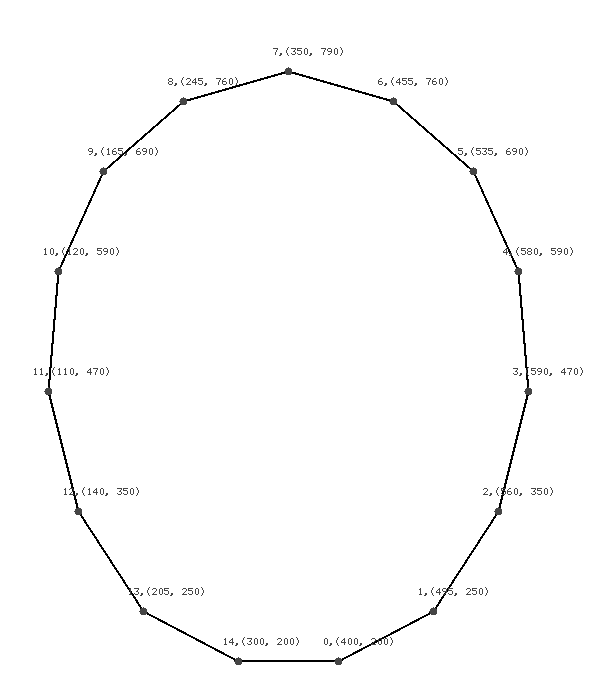
\includegraphics[scale=0.21]{fig1.png}
    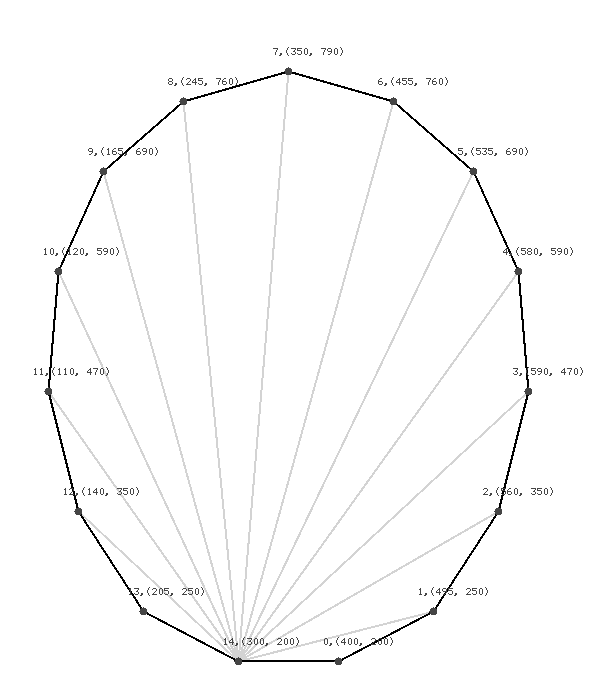
\includegraphics[scale=0.21]{fig1t.png}
    
    Fig 1 : Pentadécagone triangulé
\end{center}
\end{frame}
\begin{frame}{Introduction}
\begin{center}
    \textbf{Problématique :} Comment placer des caméras afin de couvrir une surface donnée de façon optimale ?
\end{center}
\end{frame}
%-------------------------------------------------------------------
% Le plan
\begin{frame}{Sommaire}
\tableofcontents
\end{frame}

% Pour montrer le plan avant chaque nouvelle section
\AtBeginSection[]{
  \begin{frame}{Sommaire}
  \small \tableofcontents[currentsection, hideothersubsections]
  \end{frame} 
}

%-------------------------------------------------------------------
\section{1 - Polygone convexe}
\begin{frame}{Polygone convexe}
    \begin{block}{- Définition 2}
      Un polygone P est dit convexe si l'ensemble des points dans P est un ensemble convexe, ou bien que les angles intérieurs de P sont inférieurs à $\pi$, autrement il est qualifié de concave.
    \end{block}
    \begin{center}
        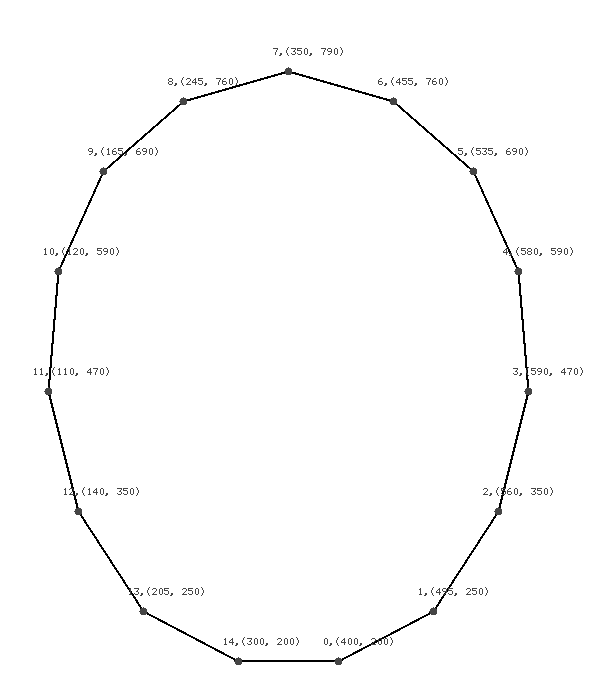
\includegraphics[scale=0.21]{fig1.png}
        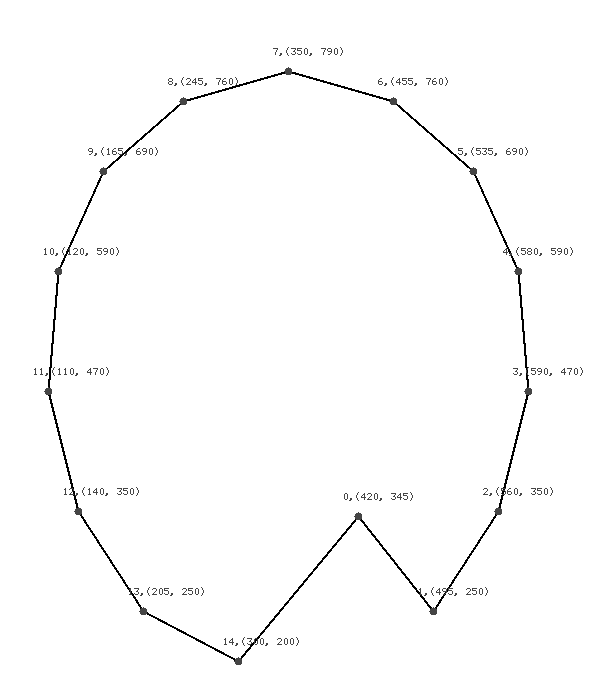
\includegraphics[scale=0.21]{figc.png}
    
         Fig 2 : Pentadécagone convexe, concave
    \end{center}
\end{frame}
%-------------------------------------------------------------------
\subsection{a) Nombre de triangulations}
    \begin{frame}{Nombre de triangulations}
        Soit $n > 2$ \newline\newline
        On pose $C_n$ le nombre de triangulations d'un polygone convexe à $n+2$ sommets. \newline
        Il est clair que $C_1 = 1$ et $C_2 = 2$.

    \begin{center}
        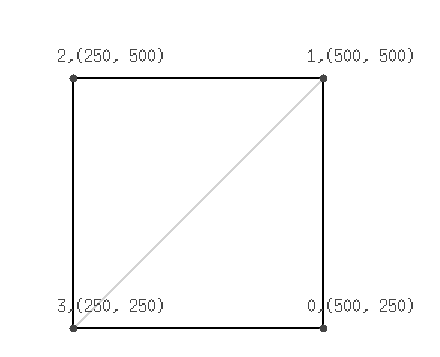
\includegraphics[scale=0.3]{square1.png}
        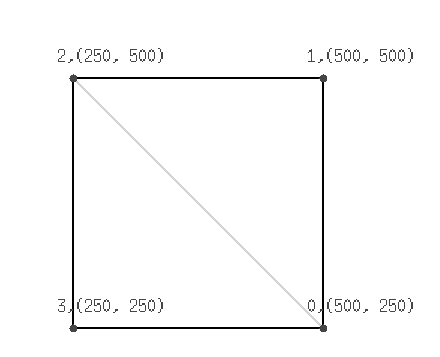
\includegraphics[scale=0.3]{square2.png}
        
        Fig 3 : Différentes triangulations d'un carré
    \end{center}
    \end{frame}
    \begin{frame}{Nombre de Triangulations}
        Cherchons une relation de récurrence permettant de calculer le nombre de triangulations d'un polygone convexe pour tout $n > 2$.\newline\newline
        Comptons-les sur l'exemple en figure 1, $n = 15$, $C_1{}_3 = $ ?.
        \begin{center}
            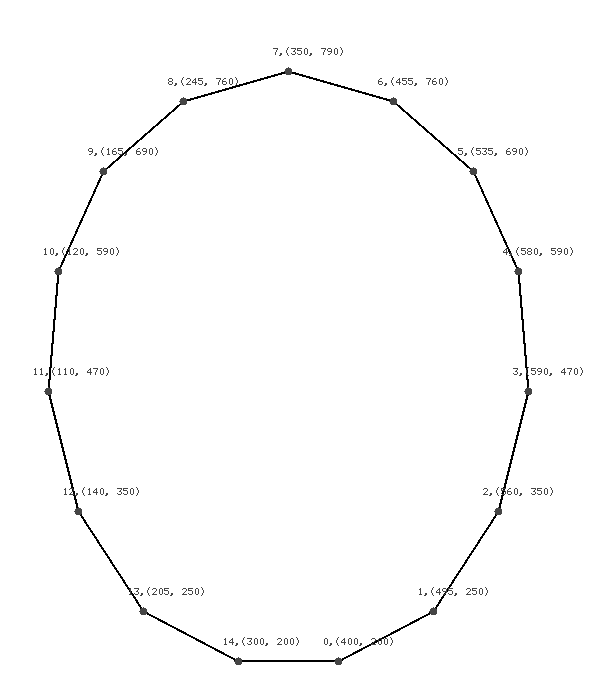
\includegraphics[scale=0.21]{fig1.png}
            
            Fig 1
        \end{center}
    \end{frame}
    \begin{frame}{Nombre de Triangulations}
        Pour cela, choisissons une arête comme base, à partir de celle-ci, on peut construire différents triangles en la reliant à un sommet du polygone. Prenons l'arête \textbf{14-0}.
        \begin{center}
            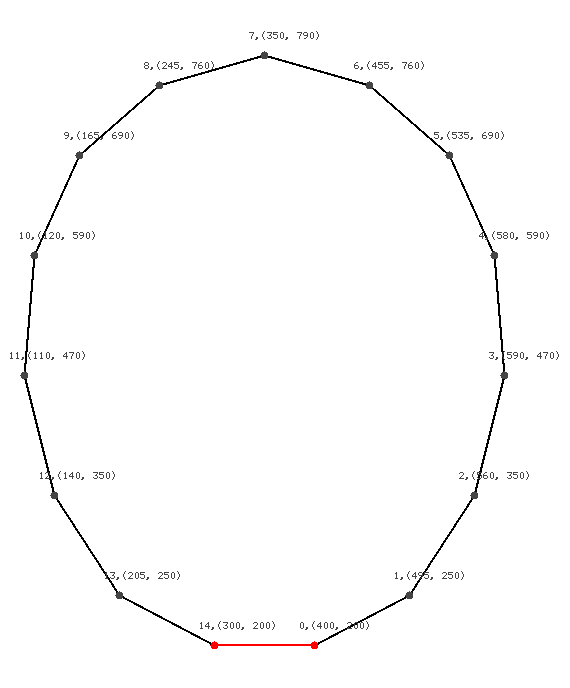
\includegraphics[scale=0.25]{cat1.png}
        \end{center}
    \end{frame}
    \begin{frame}{Nombre de Triangulations}
        Formons le triangle à l'aide du sommet \textbf{1}. \newline
        Dans ce cas, il y a $C_1{}_2$ triangulations possibles.
        \begin{center}
            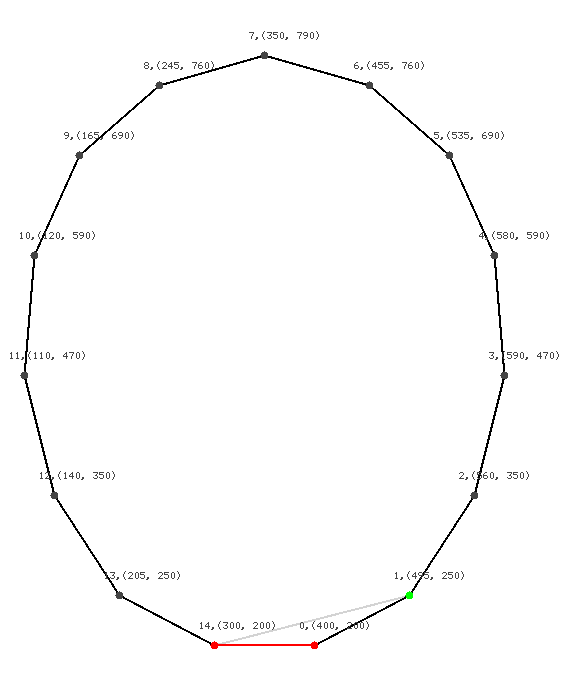
\includegraphics[scale=0.30]{cat2.png}
        \end{center}
    \end{frame}
    \begin{frame}{Nombre de Triangulations}
        Formons le triangle à l'aide du sommet \textbf{2}. \newline
        Dans ce cas, il y a $C_1{}_1C_1$ triangulations possibles.
        \begin{center}
            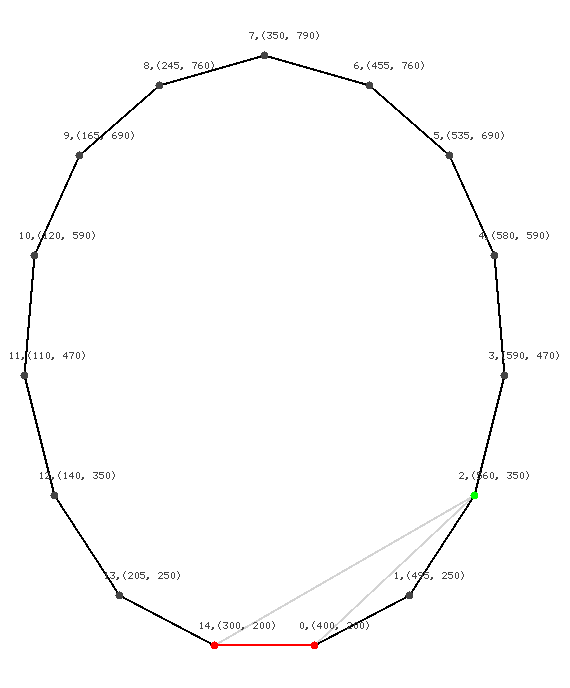
\includegraphics[scale=0.30]{cat3.png}
        \end{center}
    \end{frame}
     \begin{frame}{Nombre de Triangulations}
        Formons le triangle à l'aide du sommet \textbf{3}. \newline
        Dans ce cas il, y a $C_1{}_0C_2$ triangulations possibles.
        \begin{center}
            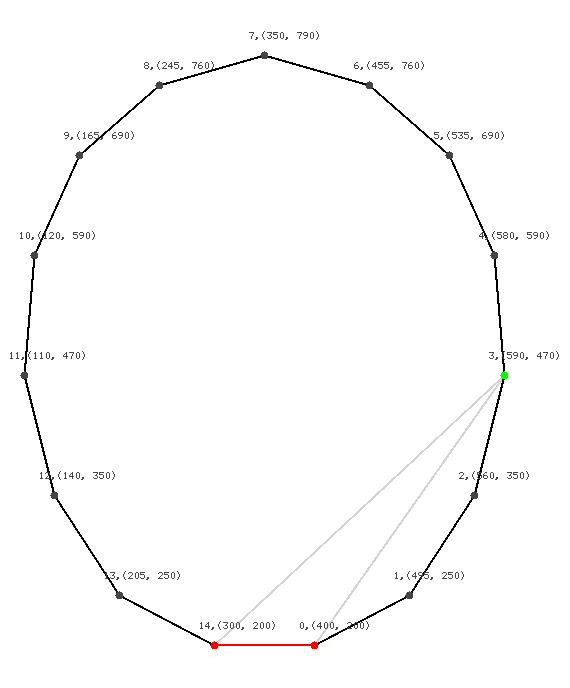
\includegraphics[scale=0.30]{cat4.png}
        \end{center}
    \end{frame}
    \begin{frame}{Nombre de Triangulations}
        Prenons la convention $C_0=1$, ainsi à chaque fois il y a $C_kC_n{}_-_k$ triangulations possibles. En sommant le tout, on obtient : \newline\newline
        \begin{equation}
            C_n_+_1 = \displaystyle  \sum_{k=0}^{n}C_kC_n_-_k
        \end{equation}
        \newline\newline
        Il s'agit de la relation de récurrence vérifiée par les nombres de Catalan.
    \end{frame}
%-------------------------------------------------------------------
\subsection{b) Nombre de Catalan}
\begin{frame}{Nombre de Catalan}
    \begin{center}{Les 18 premiers nombres de Catalan}
        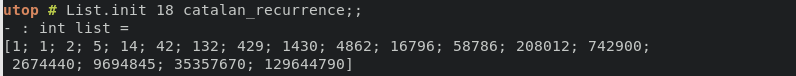
\includegraphics[scale=0.4]{catalan18.png}
        \newline
        Source : annexe
    \end{center}
\end{frame}
\begin{frame}{Nombre de Catalan}
    \begin{itemize}
        \item  Déterminons le nombre de Catalan : \newline\newline
    \end{itemize}
    On pose : $f(x) = \displaystyle  \sum_{n=0}^{\infty}C_nx^{n}$, \ $\forall x \in D(0,R)$ \newline\newline
    À l'aide d'un produit de Cauchy, on a pour $x \neq 0$ : \newline\newline
    \begin{equation}
        f(x)^{2} = \frac{f(x) - 1}{x} 
    \end{equation}
    \begin{equation}
        f(x) = \frac{1 -\sqrt{1-4x}}{2x} 
    \end{equation}
    Par continuité en 0.
\end{frame}
\begin{frame}{Nombre de Catalan}
    \begin{itemize}
        \item Par le calcul on trouve un $dse_0$ de \ $\frac{1 -\sqrt{1-4x}}{2x}$ \newline \newline
    \end{itemize}
    \begin{equation}
        \forall x \in D(0,\frac{1}{4}), \quad  \frac{1 -\sqrt{1-4x}}{2x} = \sum_{n=0}^{\infty}\frac{1}{n+1}\binom{2n}{n}x^{n}
    \end{equation}
    \newline\newline
    $C_n$ définit aussi le nombre de façons de parenthenser les mots de taille $2n$, on obtient ainsi une majoration de $C_n$, donc une minoration de son rayon $R > 0$.
\end{frame}
\begin{frame}{Nombre de Catalan}
    \begin{itemize}
        \item On obtient donc :
    \end{itemize}
     \begin{equation}
        \forall n \geqslant 0, \quad C_n = \frac{1}{n+1}\binom{2n}{n}
    \end{equation}
\end{frame}
%-------------------------------------------------------------------
\section{2 - Triangulation de polygone simple}
\begin{frame}{Polygone simple}
    \begin{block}{- Définition 3}
      Considérons un polygone P à $n$ sommets, il est dit simple si ses $n$ côtés ne se croisent pas et tels que deux côtés consécutifs n’ont qu’un seul point commun.
    \end{block}
    \begin{center}
        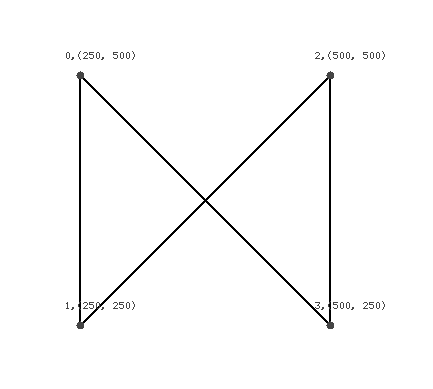
\includegraphics[scale=0.35]{!simple.png}
            
        Fig 4 polygone non simple
    \end{center}
\end{frame}
%-------------------------------------------------------------------
\subsection{a) Méthode des oreilles}
\begin{frame}{Méthode des oreilles}
    \begin{block}{- Définition 4}
      L'oreille d'un polygone est un triangle dont deux des côtés sont des cotés du polygone et dont le troisième côté est situé à l’intérieur du polygone.\newline
      \textbf{Ex :} 13.14.0 est une oreille, 14.0.1 et 0.2.3 ne le sont pas. (Fig 2)
    \end{block}
    \begin{center}
        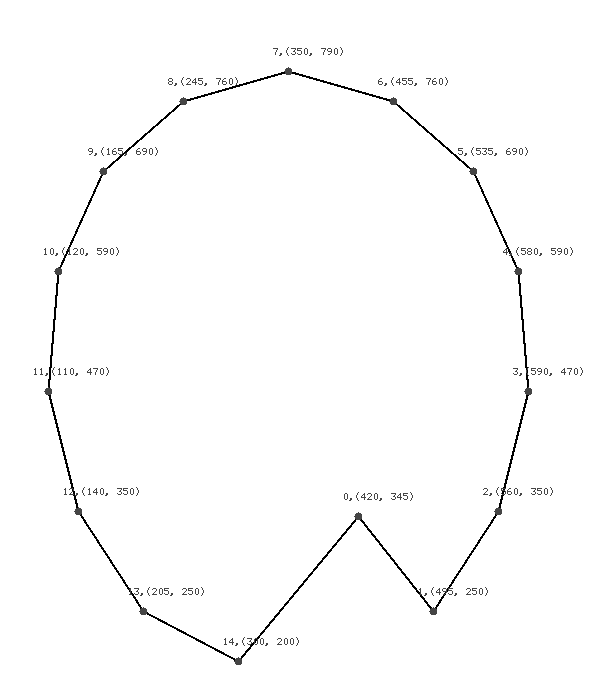
\includegraphics[scale=0.22]{figc.png}
    \end{center}
\end{frame}
\begin{frame}{Méthode des oreilles}
\begin{center}
    \begin{block}{- Proposition (admise)}
        Tout polygone simple P avec $n > 3$ sommets possède au moins 2 oreilles distinctes. \newline\newline
    \end{block}
    \begin{itemize}
        \item  De par la méthode des oreilles, il en découlera que tout polygone simple admet une triangulation de $n-2$ triangles.
    \end{itemize}
\end{center}
\end{frame}
\begin{frame}{Méthode des oreilles}
    Algorithme earclipping : \newline\newline
    Entrée : P un polygone à n sommets \newline
    Sortie : Triangulation de P sous une liste de triangle. \newline\newline
    Soit L une liste vide 
    \begin{enumerate}
        \item <1 -> On cherche une oreille A.B.C  de P qu'on ajoute dans L.
        \item <2 -> On enlève le sommet B de P.
        \item <3 -> On réitère jusqu'à triangulation.
    \end{enumerate}   
\end{frame}
\begin{frame}{Méthode des oreilles}
    \begin{center}
        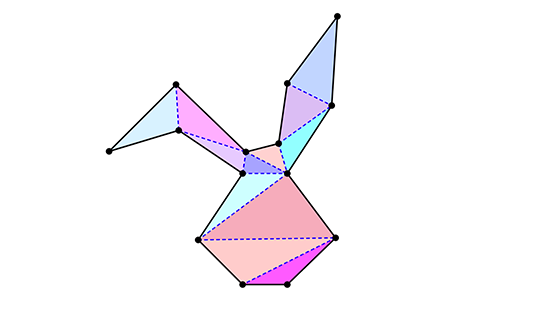
\includegraphics[scale=0.55]{oreilles.png}
        
        Fig 5 : polygone simple triangulé par amputations successives d’oreilles.
        Source : Tangente
        
    \end{center}    
\end{frame}
\begin{frame}{Méthode des oreilles}
    \begin{block}{- Définition 5}
      Un sommet est dit convexe si l'angle formé au niveau de son sommet dans P est plus petit que $\pi$ concave sinon. \newline
      \textbf{Ex :} 3 est convexe et 5 est concave.
    \end{block}
    \begin{center}
        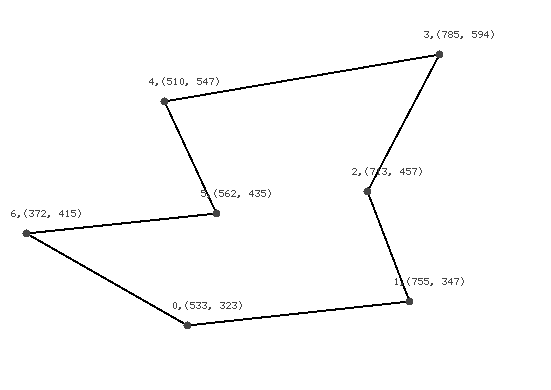
\includegraphics[scale=0.35]{sommet.png}
        
        Fig 6 : polygone simple
    \end{center}
\end{frame}
\begin{frame}[fragile]{Méthode des oreilles}
    Implémentation en Ocaml : \newline
    \begin{minted}{ocaml}
        type point = int * int 
        type polygon = point list 
        type triangle = point * point * point

        type vertex = {
        pos : point ;
        mutable convex : bool ;
        mutable concav : bool ;
        mutable ear : bool
        }
    \end{minted}   
\end{frame}
\begin{frame}{Méthode des oreilles}
    On trouve une oreille de la façon suivante : \newline\newline
    Soit 3 sommets consécutifs $v_i_-_1$, $v_i$, $v_i_+_1$, ils forment une oreille si :
    \begin{enumerate}
        \item <2-> $v_i$ est convex
        \item <3-> Aucun sommet concave du polygone n'est dans le triangle $v_i_-_1$$v_i$$v_i_+_1$ sauf possiblement $v_i_-_1$ et $v_i_+_1$     
    \end{enumerate}
\end{frame}
\begin{frame}{Méthode des oreilles}
    Comment savoir si un sommet est concave ou convexe ? \newline
    \begin{itemize}
        \item  On prend pour convention que les sommets du polygone soient cycliques et ordonnés dans le sens trigonométrique.
    \end{itemize}
   \newline    
    \begin{center}
        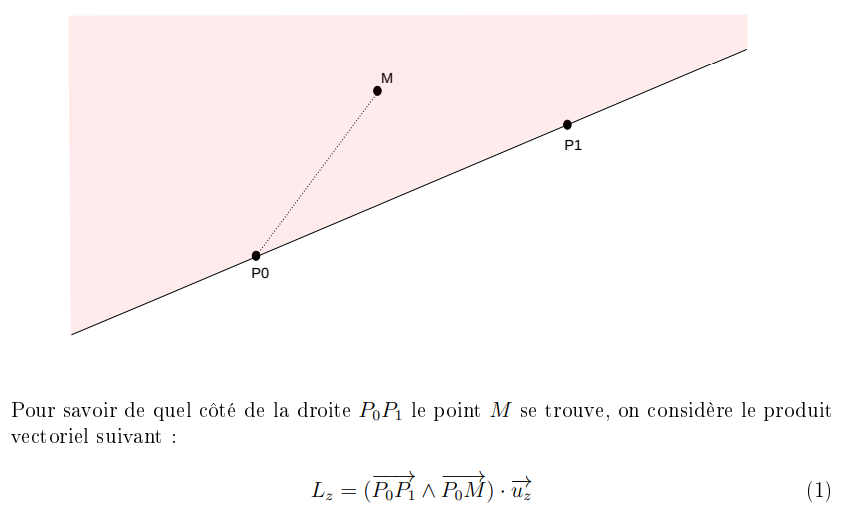
\includegraphics[scale=0.25]{vectoriel.png}
        Source : MCOT[1]
    \end{center}
\end{frame}
\begin{frame}{Méthode des oreilles}
    \begin{center}
        \begin{enumerate}
            \item $L_z > 0$ m se trouve à gauche du segment
            \item $L_z < 0$ m se trouve à droite du segment
            \item $L_z = 0$ m se trouve sur le segment \newline\newline
        \end{enumerate}
        \begin{itemize}
            \item À l'aide de $L_z$ on peut facilement savoir si un sommet est convexe, et si un point se trouve à l'intérieur d'un triangle.
        \end{itemize}
    \end{center}
\end{frame}
\begin{frame}{Méthode des oreilles}
    Complexité de l'algorithme : \newline\newline
    Entrée : P un polygone à n sommets \newline\newline
    Sortie : Triangulation de P sous une liste de triangle. \newline\newline
    Soit L une liste vide 
    \begin{enumerate}
        \item On cherche une oreille A.B.C  de P qu'on ajoute dans L. \textbf{O(n)}
        \item On enlève le sommet B de P. \textbf{O(n)}
        \item On réitère jusqu'à triangulation. ($n-3$ fois)  \textbf{O(n)} \newline\newline
    \end{enumerate}
    \begin{center}
        L'algorithme est en \textbf{O(n²)}.
    \end{center}
\end{frame}
\begin{frame}{Méthode des oreilles}
\begin{center}
    \begin{tikzpicture}
    \begin{axis}[
        title={Triangulation d'un polygone simple aléatoire à n sommets} ,
        width=1\textwidth,
        height=.8\textheight,
        xlabel = $n$ ,
        ylabel = Temps d'exécution (s),
        legend pos=north west,
        ymajorgrids=true,
        grid style=dashed]
            \addplot [color=blue, only marks, mark size = 1]table [y=temps, x=n]{complexite.txt};
            \addlegendentry{\(ear clipping\)}
            \addplot[domain=0:200, samples=90][color = red ]{x*x*10e-6};
            \addlegendentry{\( x^{2}10^{-6}\)}
    \end{axis}
    \end{tikzpicture}
\end{center}
\end{frame}
%-------------------------------------------------------------------
\subsection{b) Décomposition Monotone}
\begin{frame}{Décomposition Monotone}
    \begin{block}{- Définition 5}
     Un polygone P est dit Y (resp X) monotone si chaque droite orthogonale à l'axe Y (resp X) coupe la frontière de P au plus deux fois.
    \end{block}
    \begin{center}
        \includegraphics[scale=0.4]{figm.png}

        Fig 7 : polygone y-monotone
    \end{center}
\end{frame}
\begin{frame}{Décomposition Monotone}
    Traitons le cas des polygones y-monotones. \newline\newline
    Soit P y-monotone.\newline
    \begin{itemize}
        \item Le déplacement sur la frontière gauche ou droite de P fait en sorte que nous descendons toujours du sommet le plus élevé de P au plus bas.\newline\newline
    \end{itemize}
    Cette propriété nous permet de le trianguler en \textbf{O(n)}
\end{frame}
\begin{frame}{Décomposition Monotone}
    \begin{itemize}
        \item Partitionnement en sous-polygone monotone d'un polygone simple.
    \end{itemize}
    \begin{center}
        \includegraphics[scale=0.4]{vertex.png}
        \includegraphics[scale=0.4]{part.png}
    \end{center}
\end{frame}
\begin{frame}{Décomposition Monotone}
    \begin{block}{- Proposition}
        Tout polygone P est  y-monotone s'il ne possède ni sommet split ni sommet merge.\newline\newline 
    \end{block}
    \begin{itemize}
        \item Ainsi, le partitionnement se fait en ajoutant des diagonales depuis les sommets split et merge à l'aide d'un algorithme de ligne de balayage qui se fait en \textbf{O(nlog n)} \newline\newline
        \item La décomposition monotone est donc en \textbf{O(nlog n)}
    \end{itemize}
\end{frame}
%-------------------------------------------------------------------
\section{3 - Problème de la galerie d'art}
\begin{frame}{Problème de la galerie d'art}
    « Quel est le nombre de caméras nécessaires pour surveiller une galerie d'art, et où faut-il les placer ? » \newline\newline
    \begin{block}{- Théorème}
      Pour garder un polygone simple à $n$ sommets,  $\left \lfloor {n/3} \right \rfloor$ caméras suffisent, et cette borne peut être atteinte.
    \end{block}
\end{frame}
%-------------------------------------------------------------------
\subsection{a) 3-Coloriage}
\begin{frame}{3-Coloriage}
    \begin{block}{- Proposition (admise)}
      Tout polygone simple P à partir de sa triangulation T admet un 3-coloriage. $T = (S,A)$ avec $S$ l'ensemble des sommets de P et $A$ l'ensemble des arretes de la triangulation.
      \begin{center}
        \includegraphics[scale=0.25]{tgraphe.png}
        Fig 8 : graphe 3-colorié
    \end{center}
  \end{block}
\end{frame}
\begin{frame}{3-Coloriage}
    \begin{center}
         Ainsi, en plaçant une caméra sur chaque sommet de la même couleur, on couvre le polygone. En choisissant la couleur qui minimise le nombre de caméras, le nombre de caméras sera majoré par $\left \lfloor {n/3} \right \rfloor$.
    \end{center}
\end{frame}
\begin{frame}{3-Coloriage}
\begin{center}
    \begin{tikzpicture}
    \begin{axis}[
        title={Nombre de caméras pour un polygone simple aléatoire à n sommets} ,
        width=1\textwidth,
        height=.8\textheight,
        xlabel = $n$ ,
        ylabel = $n_c$,
        legend pos=north west,
        ymajorgrids=true,
        grid style=dashed]
            \addplot [color=blue, only marks, mark size = 1]table[y=camera, x=n]{graphe2.txt};
            \addlegendentry{\(caméras\)}
            \addplot[domain=0:200, samples=100][color = red ]{x/3};
            \addlegendentry{\(n/3\)}
    \end{axis}
    \end{tikzpicture}
\end{center}
\end{frame}
%-------------------------------------------------------------------
\subsection{b) Application}
\begin{frame}{Application}
    Plan Musée du Louvre
      \begin{center}
        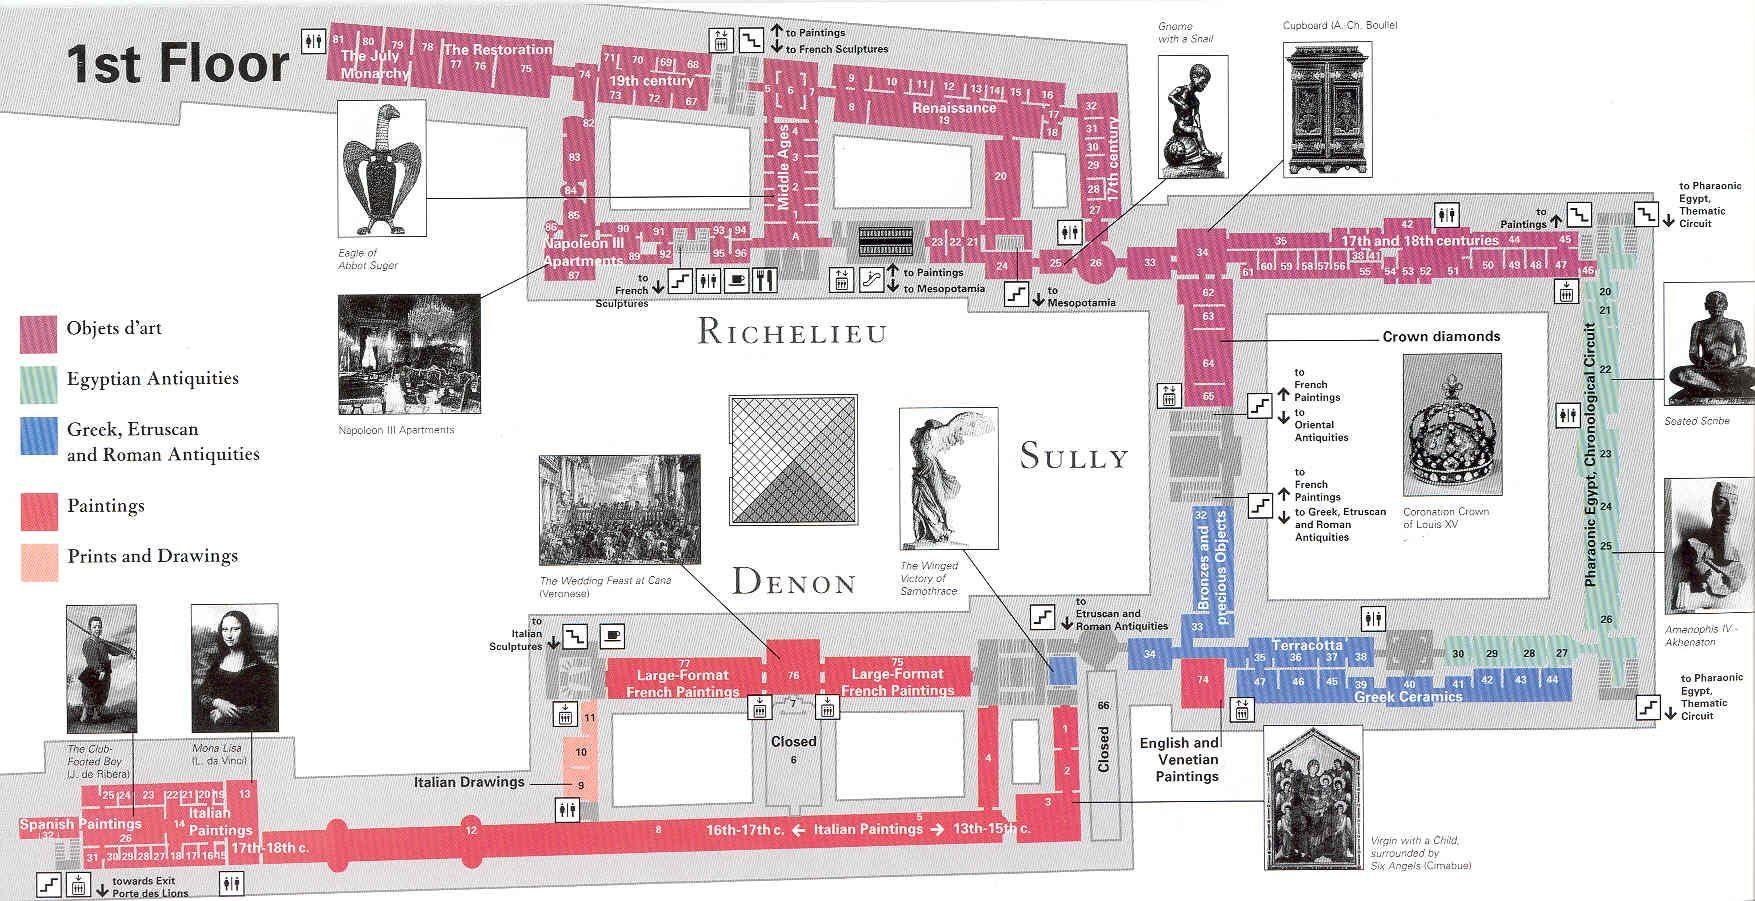
\includegraphics[scale=0.38]{plan_louvre.jpg}
        
        Source : plandeparis.info
    \end{center}
\end{frame}
\begin{frame}{Application}
    \begin{center}
        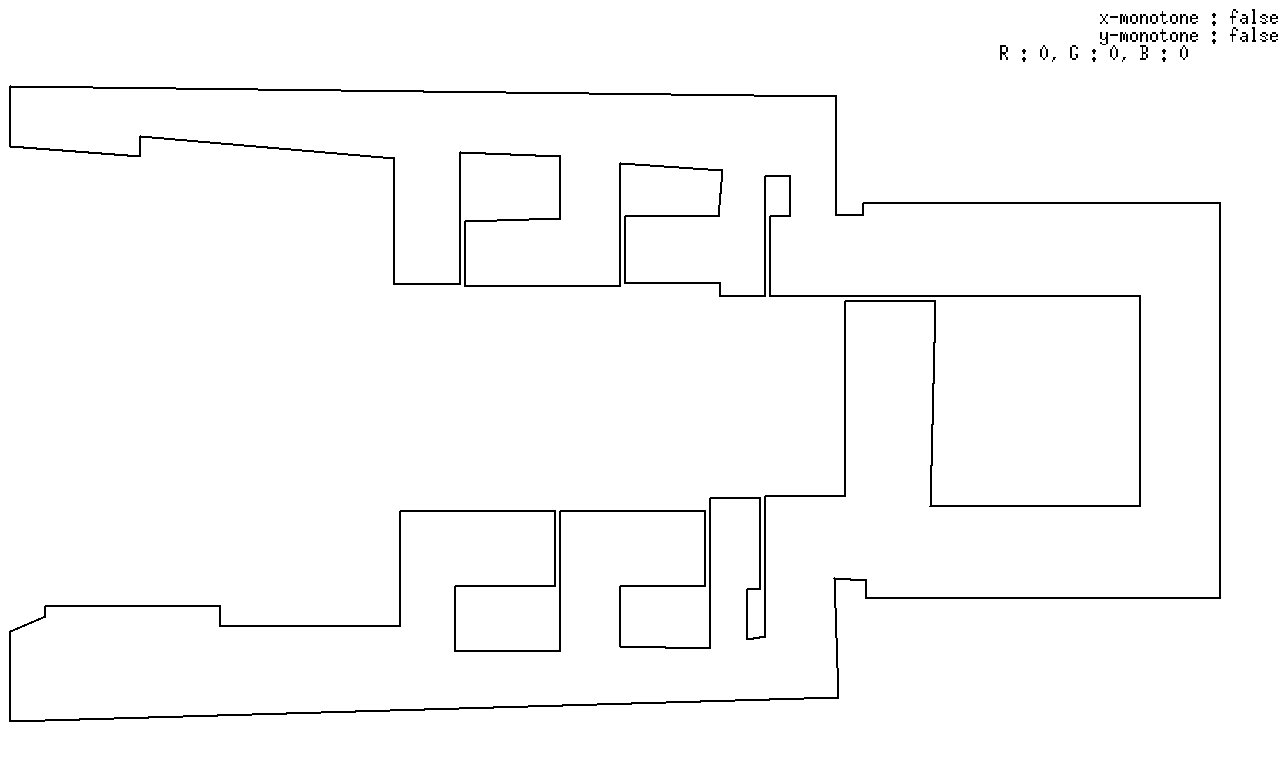
\includegraphics[scale=0.26]{louvre1.png}
    \end{center}
\end{frame}
\begin{frame}{Application}
    \begin{center}
        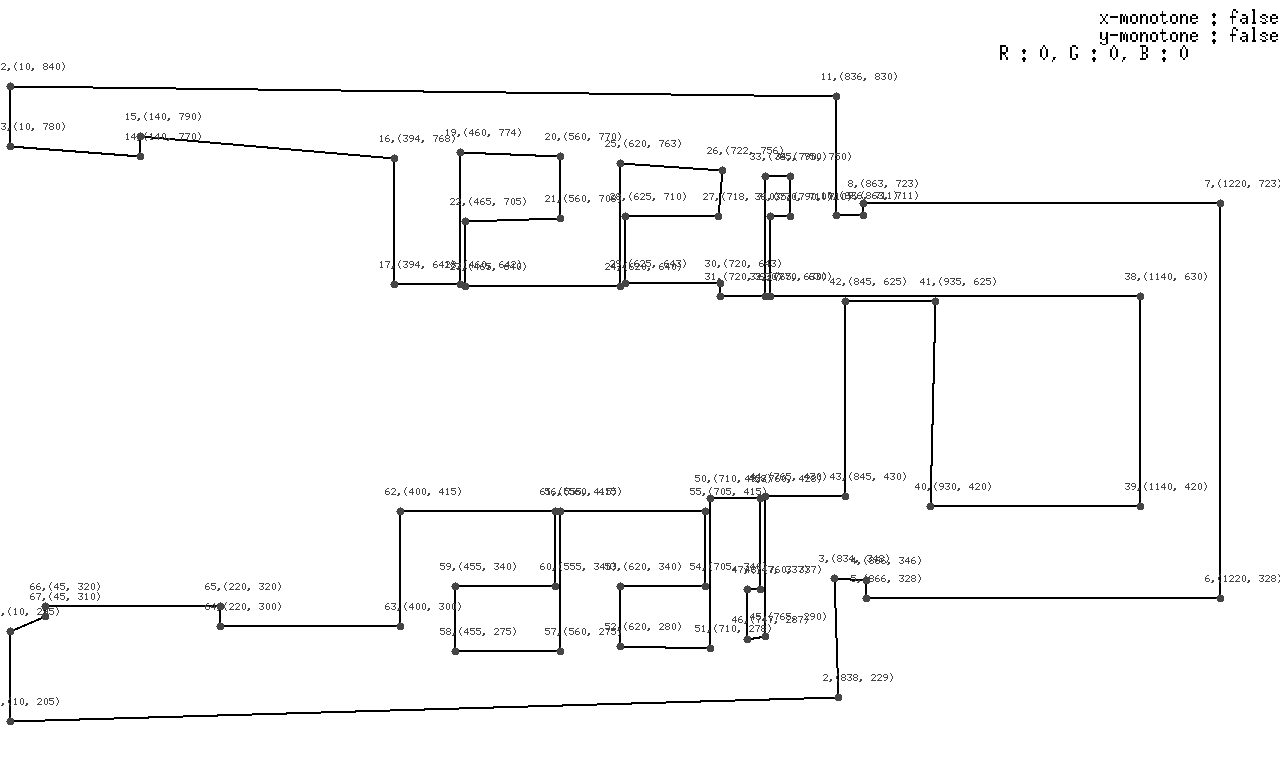
\includegraphics[scale=0.26]{louvre2.png}
    \end{center}
\end{frame}
\begin{frame}{Application}
    \begin{center}
        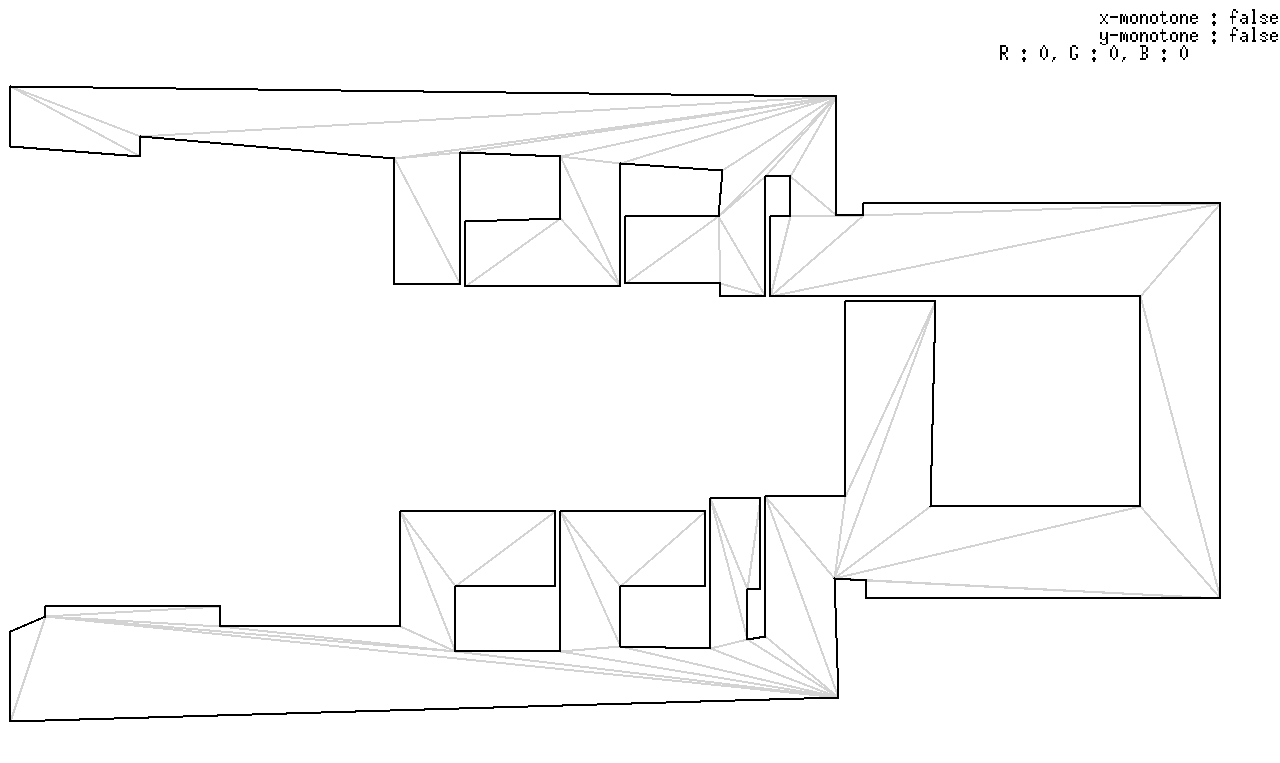
\includegraphics[scale=0.26]{louvre3.png}
    \end{center}
\end{frame}
\begin{frame}{Application}
    \begin{center}
        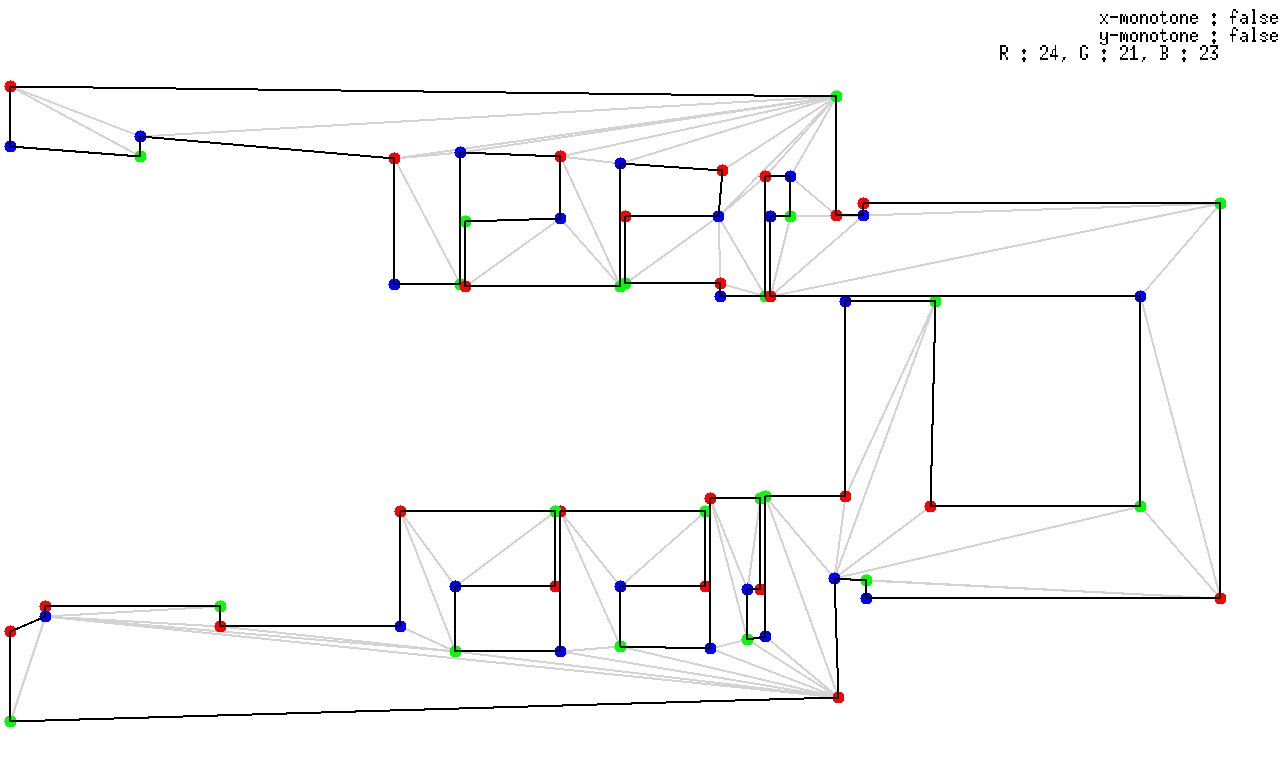
\includegraphics[scale=0.26]{louvre4.png}
    \end{center}
\end{frame}
\begin{frame}{Application}
    \begin{center}
        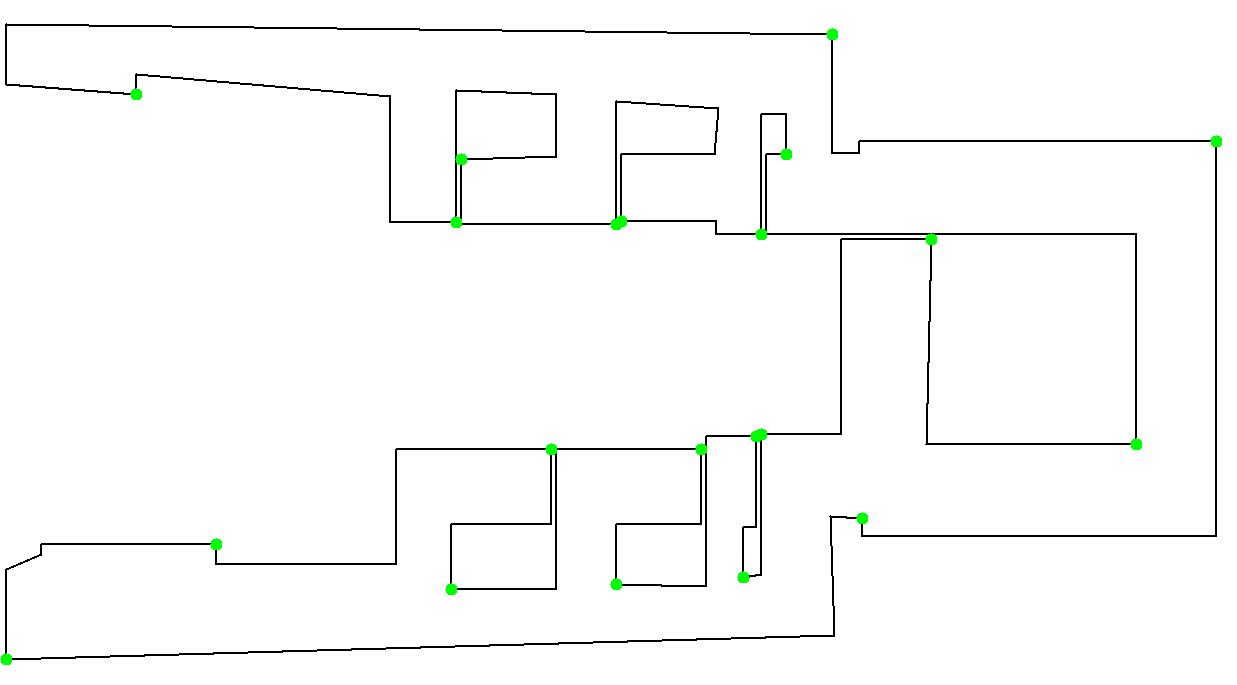
\includegraphics[scale=0.26]{louvre5.png}
        On peut se ramener à $21 - 5 = 16$ caméras pour $68 - 14 = 54$ sommets.
    \end{center}
\end{frame}
\begin{frame}{}
    \begin{center}
        MERCI\ POUR\ VOTRE\ ATTENTION 
    \end{center}    
\end{frame}
%-------------------------------------------------------------------
\section{- Annexe}
\begin{frame}{Programme Informatique}
    Liste du code utilisé : \newline \newline
    \begin{itemize}
        \item Catalan.ml
        \item Affichage.ml (fichier principal)
        \item Triangulation.ml
        \item Coloriage.ml
        \item Arbre\_BR.ml (Structure pour la décomposition monotone)
        \item random\_poly.py (Utilisé avec graphe.ml pour générer les données utiles à la présentation)
        \item graphe.ml
    \end{itemize}
\end{frame}
%-------------------------------------------------------------------
\begin{frame}{Catalan.ml}
    \begin{center}
        CATALAN.ML
    \end{center}    
\end{frame}
\inputminted[obeytabs=true,tabsize=2, breaklines, linenos, fontsize=\tiny]{ocaml}{Catalan.ml}

\begin{frame}{Affichage.ml}
    \begin{center}
        AFFICHAGE.ML
    \end{center}    
    \newline\newline 
    \textbf{fichier main} (on compile de la façon suivante : ocamlfind ocamlc -package graphics -linkpkg Arbre\_BR.ml Triangulation.ml Coloriage.ml Affichage.ml )
\end{frame}
\inputminted[obeytabs=true,tabsize=2, breaklines, linenos, fontsize=\tiny]{ocaml}{Affichage.ml}

\begin{frame}{Triangulation.ml}
    \begin{center}
        TRIANGULATION.ML 
    \end{center}    
\end{frame}
\inputminted[obeytabs=true,tabsize=2, breaklines, linenos, fontsize=\tiny]{ocaml}{Triangulation.ml}

\begin{frame}{Coloriage.ml}
    \begin{center}
        COLORIAGE.ML 
    \end{center}    
\end{frame}
\inputminted[obeytabs=true,tabsize=2, breaklines, linenos, fontsize=\tiny]{ocaml}{Coloriage.ml}

\begin{frame}{Arbre\_BR.ml}
    \begin{center}
        ARBRE\_BR.ML 
    \end{center}    
\end{frame}
\inputminted[obeytabs=true,tabsize=2, breaklines, linenos, fontsize=\tiny]{ocaml}{Arbre_BR.ml}

\begin{frame}{random\_poly.py}
    \begin{center}
        RANDOM\_POLY.PY (On met les données dans val.ml python3 random\_poly.py > val.ml)
    \end{center}    
\end{frame}
\inputminted[obeytabs=true,tabsize=2, breaklines, linenos, fontsize=\tiny]{python}{random_poly.py}

\begin{frame}{graphe.ml}
    \begin{center}
        GRAPHE.ML 
    \end{center}    
\end{frame}
\inputminted[obeytabs=true,tabsize=2, breaklines, linenos, fontsize=\tiny]{ocaml}{graphe.ml}

\end{document}
%-------------------------------------------------------------------